There are various methods available to implement image
fusion. Basically, these methods can be categorized into two
categories. The first category is the spatial domain-based methods, which directly fuse the source images into the intensity
values . The other category is the transformed domain-based methods, which fuse images with certain frequency or time frequency transforms Assuming that F(·) represents the “fusion operator,” the fusion methods in the spatial domain can be summarized as 
\begin{equation}
 {I}_{F}= F({I}_{1},{I}_{2} \dots{} {I}_{k})
\end{equation}
The simplest fusion method in spatial domain just takes
the pixel-by-pixel average of the source images. However, this
method often leads to undesirable side effects, such as reduced
contrast . If the source images are not completely registered,
then a single pixel-based method, such as spatial gradient (SG) based method, always results in artifacts in the fused
image. Therefore, some more reasonable methods were proposed to fuse source images with divided blocks or segmented
regions instead of single pixels. However, the blockbased fusion methods usually suffer from blockness in the fused image. For the region-based method, the source images are first segmented, and the obtained regions are then fused using their properties, such as spatial frequency or SG. The segmentation algorithms, usually complicated and time consuming, are of vital importance to the fusion quality.A more popular method that has been explored in recent years is by using multiscale transforms The transformed domain-based methods can be summarized as
\begin{equation}
{I}_{F}={T}^{-1}(F(T({I}_{1}),T({I}_{2})\dots{} T({I}_{j}))
\end{equation}
\hfill \break
 Because the fused image obtained by transform domain-based algorithms is globally created, a little change in a single coefficient of the fused image in the transformed domain may cause all the pixel values to change in spatial domain. As a result, undesirable artifacts may be produced in the fusion process using the multiresolution transform-based methods in some cases
Obviously, effectively and completely extracting the underlying information of the original images would make the fused image more accurate. Different from multiscale transformations, the sparse representation using an overcomplete dictionary that contains prototype signal atoms describes signals by sparse linear combinations of these atoms \cite{30-34} Two main characteristics of sparse representation are its overcompleteness and sparsity \cite{32}. Overcompleteness means that the number of basis atoms in the dictionary exceeds the number of image pixels or signal dimensions. The overcomplete dictionary that contains rich transform bases allows for more stable and meaningful representation of signals. Sparsity means that the coefficients corresponding to a signal are sparse, that is to say, only “a few descriptions” can describe or capture the significant structure information about the object of interest. Benefiting from its sparsity and overcompleteness, sparse representation theory has successfully been applied in many practical applications, including compression, denoising, feature extraction, classification, and so on \cite{32-34}. Recent studies have shown
that common image features can also be accurately described
by only a few coefficients or “a few descriptions” \cite{32}. 
In general, sparse representation is a global operation, in the sense that it is based on the gray-level content of an entire image. However, the image fusion quality depends on the accurate
representation of the local salient features of source images.
Therefore, a “sliding window” technique is adopted to achieve
better performance in capturing local salient features and keeping shift invariance.

\section{Sparse Representaion}
SR assumes that the signal \(Y \in {\textbf{R}}^{n}\) can be represented as a linear combination of given atoms.These atoms consist of an overcomplete dictionary \( D\in {\textbf{R}}^{n*k} 
, with n<<K \). The representation of y may either be exact \(D\theta=y \) or approximate \(|D\theta -y|\leq \epsilon \)  where 
\(\epsilon \) is the specified error.The details about dictionary D is discuss in following section. The vector \(\theta \in {\textbf{R}}^{k} \) is the coefficients of the signal. The coefficients with the fewest number of nonzero coefficients is certainly an appealing representation. Exact determination of the sparsest representation proves to be an non-deterministic polynomial time-hard problem.
Approximate solutions are considered instead. Basically, two approaches were proposed in previous researches. One approach is based on greedy algorithms such as Matching Pursuit (MP) and Orthogonal Matching Pursuit (OMP).All of these approaches are based on replacing the \({l}_{0} \) with the \( { l}_{p} \) -norm,where \({l}_{p}\) (0<p≤1) is defined as \({\parallel \theta \parallel}_{p}={\left(\sum_{i} { \mid {\theta }_{i}\mid}^{p} \right)}^{1/p}  \) \hfill \break

Let  \({Y}_{i} \in {\textbf{R}}_{n*L} \left(i=1,2,....\lambda \right) \) denote the L signals with dimension from the i’th sensor. We can represent \({Y}_{i}\) with common component \(\Theta c \in {\textbf{R}}^{K*L} \) and innovation component \(\Theta_{i}^{u} \in {\textbf{R}}^{k*L}  \)of sparse coefficient matrix,and noise \({n}_{i} \in {\textbf{R}}^{n*L} \).

\begin{equation}
{Y}_{i}={Y}^{c}+Y_{i}^{u}=D{\Theta}^{c}+D\Theta_{i}^{u}+{n}_{i}
\end{equation} 

\hfill \break The concatenated source images matrix can be represented sparsely by the concatenated coefficient matrix.
\begin{equation}\label{eq:3.2}
\begin{pmatrix}
{Y}_{1}  \\ 
{Y}_{2}\\ 
\vdots\\
{Y}_{\Lambda }
\end{pmatrix}=\begin{pmatrix}
D & D & 0 & \dots{} &0 \\ 
 D& 0 &D  & \dots{} & 0 \\ 
 \vdots{}& \vdots{}  &  \vdots{} & \vdots{}  & \vdots{} \\ 
 D& 0 & 0 & \dots{} & D 
\end{pmatrix}\begin{pmatrix}
{\Theta }^{c}\\ 
\Theta _{l}^{u}\\ 
 \vdots{}      \\ 
\Theta _{\Lambda }^{u}
\end{pmatrix}+\begin{pmatrix}
{n}_{1} \\ 
{n}_{2} \\ 
\vdots{} \\ 
{n}_{\Lambda }
\end{pmatrix}
\end{equation}
where \(D \in {\textbf{R}}^{n*K} \)is the overcomplete dictionary which shared by both the common component and the innovation
component. Let  \( Y= \begin{pmatrix}
{Y}_{1}  \\ 
{Y}_{2}\\ 
\vdots\\
{Y}_{\Lambda }
\end{pmatrix} \)   \\   \(D= \begin{pmatrix}
D & D & 0 & \dots{} &0 \\ 
 D& 0 &D  & \dots{} & 0 \\ 
 \vdots{}& \vdots{}  &  \vdots{} & \vdots{}  & \vdots{} \\ 
 D& 0 & 0 & \dots{} & D 
\end{pmatrix} \) , \(\Theta=\begin{pmatrix}
{\Theta }^{c}\\ 
\Theta _{l}^{u}\\ 
 \vdots{}      \\ 
\Theta _{\Lambda }^{u}
\end{pmatrix}  \), \(n=\begin{pmatrix}
{n}_{1} \\ 
{n}_{2} \\ 
\vdots{} \\ 
{n}_{\Lambda }
\end{pmatrix} \) \\

Then, Eq \ref{eq:3.2} can be rewritten as follows
\begin{equation}
Y=D\Theta+n
\end{equation}

A crucial step of the SR/JSR is the selection of such a dictionary D. Predefined basis functions like curvelets, bandlets, variants of wavelets, etc., can be used. However, the success of such prespecified dictionaries is often limited by their suitability in capturing the structure in the signals under consideration. For example, image contents have SR over wavelet dictionary, but audio signals are better represented by sinusoids.  A more generalized approach is to learn the basis vectors that are specialized in representing the signal in question.  Several algorithms available in the literature deal with this problem, such as the K-SVD algorithm, the method of optimal directions (MOD), and the
Majorization method \cite{9,12,13} The K-SVD algorithm is slow
due to the SR computation and SVD operation exists at
its each iteration.
 \hfill \break
 The MOD does the most natural thing as \(\hat{D}=arg {min}_{D}\parallel Y-DX\parallel _{F}^{2}=Y{X}^{T} {\left(X{X}^{T}\right)}^{-1}\) However, \(X{X}^{T}\) may not be always with full rank. The Majorization method, for the dictionary update, is slow due to using the“Landweber”update (which is a gradient descent update)
as described in Ref \cite{14} 

\section{SR for Image Fusion} 

Since the sparse representation globally handles an image,
it cannot directly be used with image fusion, which depends
on the local information of source images. In my method, we
divide the source images into small patches and use the fixed
dictionary D with small size to solve this problem. In addition,
a sliding window technique is adopted to make the sparse
representation shift invariant, which is of great importance to
image fusion.
\hfill \break
We assume that source image I is divided into many image
patches. As shown in Fig.\ref{fig3.1}, to facilitate the analysis, the $\big(j^{th} \big) $ patch with size $ n×n $ is lexicographically ordered as a vector \({V}^{j}\). Then, \({V}^{j}\) can be expressed as
\begin{equation}
{V}^{j}=\sum_{t=1}^{T} {S}^{j} \left(t\right){d}_{t}
\end{equation}

where \({d}_{t}\) is an atom from a given overcomplete dictionary, and \(D\left[[{d}_{1} \dots{} {d}_{t} \dots{} {d}_{T} \right]\), which contains T atoms.\({S}_{j} = [{s}_{j}\left(1\right) \dots{} {s}_{j}\left( t\right) \dots{} {s}_{j}(T)]\)
 is the sparse representation

Assume that the vectors responding to all the patches in
image I are constituted into one matrix V. Then, Vcan be
expressed as 
\begin{equation}\label{eq:3.5}
D= \left[{d}_{1},{d}_{2} \dots{} {d}_{T}\right] \begin{pmatrix}
{S}^{1}(1) & {S}^{2}(1) & \dots{} & {S}^{j}(1) \\ 
 {S}^{1}(2)& {S}^{2}(2) & \dots{}  & {S}^{j}(2) \\ 
 \vdots{}& \vdots{}  &  \vdots{} & \vdots{}   \\ 
 {S}^{1}(T)& {S}^{2}(T) &  \dots{} & {S}^{j}(T) 
\end{pmatrix}
\end{equation}
where J is the number of image patches. Let \(S=[{s}^{1},{s}^{2},....,{s}^{j}]\). Then, eq. \ref{eq:3.5} can be expressed as 
\begin{equation}
V=DS
\end{equation}

\begin{figure}[h]
  \centering
  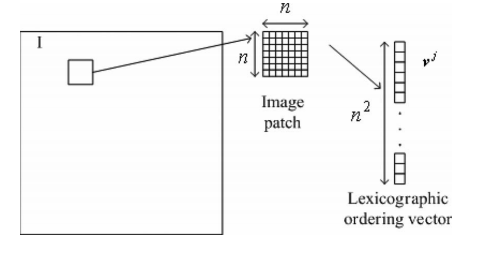
\includegraphics[width=0.5\linewidth]{3a.png}
  \label{fig3.1}
  \caption{Selected image patch and its lexicographic ordering vector.}
\end{figure}

\begin{figure}[h]
  \centering
  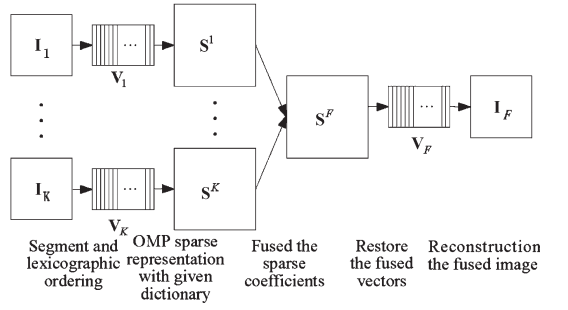
\includegraphics[width=0.5\linewidth]{3b.png}
  \label{figsr}
  \caption{Schematic diagram of the proposed SR-based fusion method.}
\end{figure}

where S is a sparse matrix.

\section{Training Dataset}
The Dictionary D is learnt from a database consisting of different type of multifocus images like medical image, infrared images, etc.
\hfill \break

I first randomly assign value in dictionary D of size \(64*256 \) from the image patches of training dataset image then i do sparse coding to get the sparse matrix of signal then i run K-SVD algorithm to update the dictionary.
\hfill \break

The training data consists of 100,000 \(8*8\)
patches, which are randomly sampled from a database of 40
high-quality natural images. The dictionary size is set to 256 and
the iteration number of K-SVD is fixed to 180.







